%Every document starts with a documentclass. 
\documentclass[11pt]{article}

%Graphicx is used to include pictures in LaTeX files. 
\usepackage{graphicx}

%The AMS packages. They contain a lot of useful math-related goodies.
\usepackage{amsthm}
\usepackage{amsmath}
\usepackage{amsfonts}
\usepackage{mdframed}
\usepackage[bottom]{footmisc}
\usepackage{bbding}
\usepackage{tcolorbox}
\usepackage{mathabx}

%This package changes the margins (makes them smaller than the default). 
\usepackage[margin=1in]{geometry}
\setlength{\headheight}{25.2pt}

%This package gives flexibility to use lettered lists in addition to numbered lists
\usepackage[shortlabels]{enumitem}

%These commands will help us define sets
\newcommand{\mn}{\mathbb{N}}
\newcommand{\mz}{\mathbb{Z}}
\newcommand{\mq}{\mathbb{Q}}
\newcommand{\mr}{\mathbb{R}}
\newcommand{\me}{\mathbb{E}}
\newcommand{\heart}{\ensuremath\heartsuit}
\newcommand{\<}{\langle}
\renewcommand{\>}{\rangle}
\newcommand\Tau{\mathcal{T}}

%The amsthm package lets you format different types of mathematical ideas nicely. You use it by defining "\newtheorem"s as below:
\newtheorem{problem}{Problem}[section]
\definecolor{myviolet}{RGB}{170, 215, 255}
\newmdenv[%
    rightmargin=0,
    backgroundcolor=myviolet,
    linewidth=1pt,
    fontcolor=black%
]{fcolor}

\newenvironment{fprob}
  {\begin{fcolor}\begin{problem}}
  {\end{problem}\end{fcolor}}

\newtheorem{theorem}{Theorem}
\newtheorem*{proposition}{Proposition}
\newtheorem*{summary}{Summary}
\newtheorem{lemma}[theorem]{Lemma}
\newtheorem{corollary}[theorem]{Corollary}
\theoremstyle{definition}
\newtheorem{defn}[theorem]{Definition}
\renewcommand*{\proofname}{Solution} %This command changes "Proof" to "Solution" in the proof environment. 

%The "\newcommand" command lets you specify a custom command. This should be used wisely to add semantic meaning to otherwise confusing sequences of commands - not just speed up typing. (If you want suggestions for shortcuts you can ask Thayer).
%Here is an example definition of a bra and ket from Quantum Mechanics.
\newcommand{\bra}[1]{\langle #1 |}
\newcommand{\ket}[1]{| #1 \rangle}
%\renewcommand\qedsymbol{\Peace}
 \renewcommand{\abstractname}{Acknowledgements:}
%Adding your name here lets you make sure every page has your name, so that your psets don't get mixed up.
\usepackage{fancyhdr}
\pagestyle{fancy}
\lhead{Connor Marrs}
\rhead{\thepage}

\title{Topology Review Summer 2021\\Problem Sets}
\date{Monday, May 17, 2021}
\author{Written by Connor Marrs\\for Professor Taback}

%This changes removes indentation and instead adds space between paragraphs. I think it looks nicer this way. 
\setlength{\parindent}{0pt}
\setlength{\parskip}{1.25ex}

%Everything above here is just commands which don't create any main-document text directly.
%You have to put all your writing within \begin{document} and \end{document} clauses.
\begin{document}
\begin{titlepage}
% \noindent\rule{\textwidth}{1pt}
\maketitle
\noindent\rule{\textwidth}{1pt}
\begin{abstract}
    These solutions are my own work, and I certify that I have consulted no unauthorized resources.
\end{abstract} 
\noindent\rule{\textwidth}{1pt}

 \begin{center}
    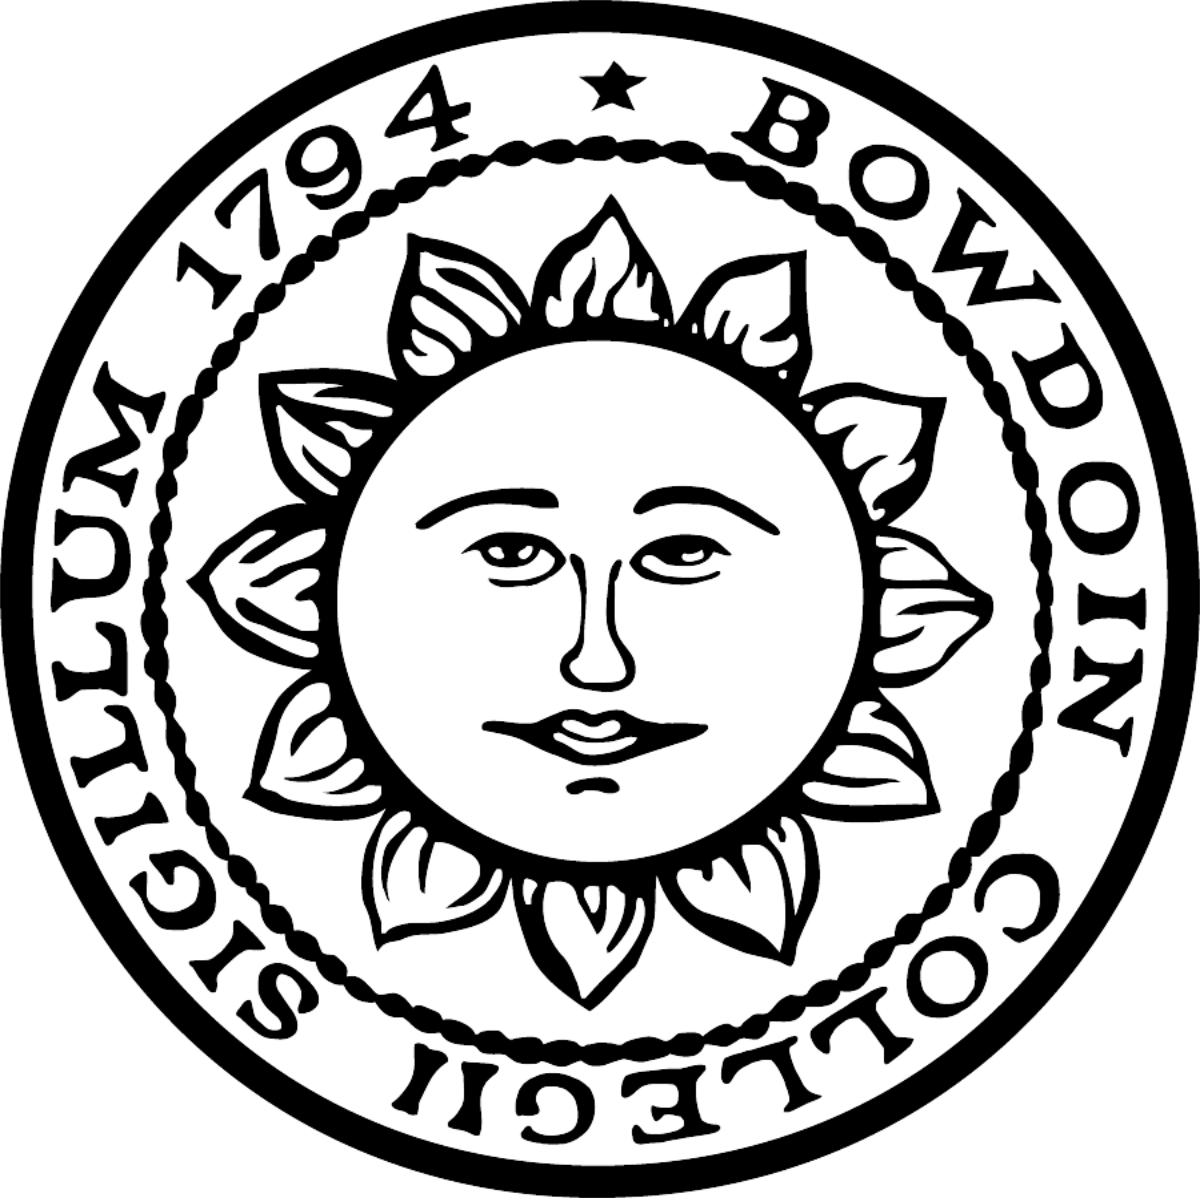
\includegraphics[scale = 0.15]{Bowdoin_Seal.png}
\end{center}

\end{titlepage}

\section{Solutions}
%%%%%%%%%%%%%%%%%%%%%%%%% PROBLEM 1.1 %%%%%%%%%%%%%%%%%%%%%%%%
\begin{fprob}
    Recall that a subset U of a metric space is open if, for all $x\in U$, there exists some
    $\varepsilon >0$ such that $B_{\varepsilon}(x)$. Show that any open ball $B_r(p)$ is in fact an open set.
\end{fprob}
\begin{proof}
    %TODO
\end{proof}

%%%%%%%%%%%%%%%%%%%%%%%%% PROBLEM 1.2 %%%%%%%%%%%%%%%%%%%%%%%%
\begin{fprob}
    Show that the collection of open sets in a metric space X satisfies the axioms of a topology, namely:
    \begin{enumerate}
        \item $\emptyset$ and $X$ are open;
        \item if $\{U_\alpha\}_{\alpha\in A}$ is an arbitrary collection of open sets, 
        then $\bigcup_{\alpha\in A}U_\alpha$ is open;
        \item if $U_1, \dots, U_n$ are open, then the intersection $\bigcap_{i=1}^nU_i$ is open.
    \end{enumerate}
    Finally, show with three examples that the arbitrary intersection of open sets is not necesarily open.
\end{fprob}

\begin{proof}
    %TODO
\end{proof}

%%%%%%%%%%%%%%%%%%%%%%%%% PROBLEM 1.3 %%%%%%%%%%%%%%%%%%%%%%%%
\begin{fprob}
    \begin{enumerate}[(a)]
        \item Show that a sequence $\{p_i\}_{i\in\mn}$ in a metric space converges 
        to a limit $p$ if and only if every open set containing $p$ also contains $p_i$ 
        for all but finitely many $i$.
        \item Show that a sequence $\{p_i\}_{i\in\mn}$ in a metric space has at most one limit.
    \end{enumerate}
\end{fprob}

\begin{proof}
    %TODO
\end{proof}

%%%%%%%%%%%%%%%%%%%%%%%%% PROBLEM 1.4 %%%%%%%%%%%%%%%%%%%%%%%%
\begin{fprob}
    Show that, if a sequence in a metric space converges to a limit, then it is a Cauchy
    sequence. Show (by giving an example) that the converse is not true.
\end{fprob}

\begin{proof}
    %TODO
\end{proof}

%%%%%%%%%%%%%%%%%%%%%%%%% PROBLEM 1.5 %%%%%%%%%%%%%%%%%%%%%%%%
\begin{fprob}
    Given any two points $p = (p_1,\dots,p_n)$ and $q = (q_1,\dots, q_n)$ in $\mr^n$, define
    \[
        d_\infty(p,q) = \max\{|p_i-q_i|, i\in\mn_n\}  
    \]
    \begin{enumerate}[(a)]
        \item Show that $(\mr^n,d_\infty)$ is a metric space.
        \item Show that a subset of $\mr^n$ is open in $(\mr^n,d_\infty)$ if and only if it is open 
        for the Euclidean distance $(\mr^n,d)$. (In other terms: $d$ and $d_\infty$ induce the same 
        topology on $\mr^n$).
    \end{enumerate}
\end{fprob}

\begin{proof}
    %TODO
\end{proof}


%%%%%%%%%%%%%%%%%%%%%%%%% PROBLEM 1.6 %%%%%%%%%%%%%%%%%%%%%%%%
\begin{fprob}
    Let $X$ be any set. For $p,q\in X$ and define $d(p,q)=\begin{cases} 1 & p\neq q \\ 0 & p=q\end{cases}$.
    Prove that this is a metric. Which subsets of the metric space $(X,d)$ are open, and which are closed?
\end{fprob}

\begin{proof}
    %TODO
\end{proof}


\end{document}